% Options for packages loaded elsewhere
\PassOptionsToPackage{unicode,backref,colorlinks=true}{hyperref}
\PassOptionsToPackage{hyphens}{url}
%
\documentclass[
  10pt,
  a4paper,
]{article}
\usepackage{amsmath,amssymb}
\usepackage[]{tgpagella}
\usepackage{ifxetex,ifluatex}
\ifnum 0\ifxetex 1\fi\ifluatex 1\fi=0 % if pdftex
  \usepackage[T1]{fontenc}
  \usepackage[utf8]{inputenc}
  \usepackage{textcomp} % provide euro and other symbols
\else % if luatex or xetex
  \usepackage{unicode-math}
  \defaultfontfeatures{Scale=MatchLowercase}
  \defaultfontfeatures[\rmfamily]{Ligatures=TeX,Scale=1}
\fi
% Use upquote if available, for straight quotes in verbatim environments
\IfFileExists{upquote.sty}{\usepackage{upquote}}{}
\IfFileExists{microtype.sty}{% use microtype if available
  \usepackage[]{microtype}
  \UseMicrotypeSet[protrusion]{basicmath} % disable protrusion for tt fonts
}{}
\makeatletter
\@ifundefined{KOMAClassName}{% if non-KOMA class
  \IfFileExists{parskip.sty}{%
    \usepackage{parskip}
  }{% else
    \setlength{\parindent}{0pt}
    \setlength{\parskip}{6pt plus 2pt minus 1pt}}
}{% if KOMA class
  \KOMAoptions{parskip=half}}
\makeatother
\usepackage{xcolor}
\IfFileExists{xurl.sty}{\usepackage{xurl}}{} % add URL line breaks if available
\IfFileExists{bookmark.sty}{\usepackage{bookmark}}{\usepackage{hyperref}}
\hypersetup{
  pdftitle={Submodels, priors, and pooling the link parameters in the survival example},
  pdfauthor={Andrew Manderson},
  hidelinks,
  pdfcreator={LaTeX via pandoc}}
\urlstyle{same} % disable monospaced font for URLs
\usepackage[margin=2.25cm]{geometry}
\usepackage{graphicx}
\makeatletter
\def\maxwidth{\ifdim\Gin@nat@width>\linewidth\linewidth\else\Gin@nat@width\fi}
\def\maxheight{\ifdim\Gin@nat@height>\textheight\textheight\else\Gin@nat@height\fi}
\makeatother
% Scale images if necessary, so that they will not overflow the page
% margins by default, and it is still possible to overwrite the defaults
% using explicit options in \includegraphics[width, height, ...]{}
\setkeys{Gin}{width=\maxwidth,height=\maxheight,keepaspectratio}
% Set default figure placement to htbp
\makeatletter
\def\fps@figure{htbp}
\makeatother
\setlength{\emergencystretch}{3em} % prevent overfull lines
\providecommand{\tightlist}{%
  \setlength{\itemsep}{0pt}\setlength{\parskip}{0pt}}
\setcounter{secnumdepth}{5}
\usepackage{amsmath}
% I always seem to need tikz for something
\usepackage{tikz}
\usetikzlibrary{positioning, shapes, intersections, through, backgrounds, fit, decorations.pathmorphing, angles, quotes}
\usepackage{setspace}
\onehalfspacing

\usepackage{lineno}
% \linenumbers

\usepackage{relsize}
\usepackage{placeins}

% required for landscape pages. beware, they back the build very slow.
\usepackage{pdflscape}

% table - `gt' package uses these, often unimportant
\usepackage{longtable}
\usepackage{booktabs}
\usepackage{caption}

\usepackage{color}
\definecolor{myredhighlight}{RGB}{180, 15, 32}
\definecolor{mydarkblue}{RGB}{0, 33, 79}
\definecolor{mymidblue}{RGB}{44, 127, 184}
\definecolor{mylightblue}{RGB}{166, 233, 255}

\usepackage{colortbl}

\newcommand{\semitransp}[2][35]{\color{fg!#1}#2}

\setcounter{secnumdepth}{3}

\let\Oldcap\cap
\renewcommand{\cap}{\mathrel{\mathsmaller{\Oldcap}}}

% pd stands for: probability distribution and is useful to distringuish
% marignals for probabilities specifically p(p_{1}) and the like.
\newcommand{\pd}{\text{p}}
\newcommand{\q}{\text{q}}
\newcommand{\w}{\text{w}}
\newcommand{\pdr}{\text{r}}
\newcommand{\pdrh}{\hat{\text{r}}}

% melding
\newcommand{\ppoolphi}{\pd_{\text{pool}}(\phi)}
\newcommand{\pmeld}{\pd_{\text{meld}}}

% the q(x)w(x), "weighted target" density 
% for the moment I'm going to call it s(x), as that is the next letter of the 
% alphabet. Can change it later
\newcommand{\s}{\text{s}}
% direct density estimate - replaces lambda.
\newcommand{\ddest}{\text{s}}
% target weighting function
\newcommand{\tarw}{\text{u}}

% constants - usually sizes of things
\newcommand{\Nx}{N}
\newcommand{\Nnu}{\text{N}_{\text{nu}}}
\newcommand{\Nde}{\text{N}_{\text{de}}}
\newcommand{\Nmc}{\text{N}_{\text{mc}}}
\newcommand{\Nw}{W}
\newcommand{\Nm}{M}
\newcommand{\Ns}{S}
\newcommand{\Np}{P}

% locales - could switch to x and x'
\newcommand{\xnu}{x_{\text{nu}}}
\newcommand{\xde}{x_{\text{de}}}
\newcommand{\phinu}{\phi_{\text{nu}}}
\newcommand{\phide}{\phi_{\text{de}}}

% sugiyama stuff
\newcommand{\pdnu}{\pd_{\text{nu}}}
\newcommand{\pdde}{\pd_{\text{de}}}

% indices 
\newcommand{\wfindex}{w}
\newcommand{\sampleindex}{n}
\newcommand{\modelindex}{m}
\newcommand{\stageindex}{s}
\newcommand{\phiindex}{p}

% independence symbol
\newcommand{\indep}{\perp\!\!\!\perp}
\newcommand{\setcomp}{\mathsf{c}}

\newtheorem{theorem}{Theorem}[section]
\newtheorem{corollary}{Corollary}[theorem]

\DeclareMathOperator*{\argmin}{arg\,min}

% ARDS example in text commands
\newcommand{\paoii}{PaO\textsubscript{2}}
\newcommand{\fioii}{FiO\textsubscript{2}}
\newcommand{\spoii}{SpO\textsubscript{2}}
\newcommand{\pfratio}{\paoii/\fioii}
\newcommand{\sfratio}{\spoii/\fioii}
\ifluatex
  \usepackage{selnolig}  % disable illegal ligatures
\fi
\newlength{\cslhangindent}
\setlength{\cslhangindent}{1.5em}
\newlength{\csllabelwidth}
\setlength{\csllabelwidth}{3em}
\newenvironment{CSLReferences}[2] % #1 hanging-ident, #2 entry spacing
 {% don't indent paragraphs
  \setlength{\parindent}{0pt}
  % turn on hanging indent if param 1 is 1
  \ifodd #1 \everypar{\setlength{\hangindent}{\cslhangindent}}\ignorespaces\fi
  % set entry spacing
  \ifnum #2 > 0
  \setlength{\parskip}{#2\baselineskip}
  \fi
 }%
 {}
\usepackage{calc}
\newcommand{\CSLBlock}[1]{#1\hfill\break}
\newcommand{\CSLLeftMargin}[1]{\parbox[t]{\csllabelwidth}{#1}}
\newcommand{\CSLRightInline}[1]{\parbox[t]{\linewidth - \csllabelwidth}{#1}\break}
\newcommand{\CSLIndent}[1]{\hspace{\cslhangindent}#1}

\title{Submodels, priors, and pooling the link parameters in the
survival example}
\author{Andrew Manderson}
\date{19 May, 2021}

\begin{document}
\maketitle

\hypertarget{models}{%
\section{Models}\label{models}}

There are \(i = 1, \ldots, N\) individuals (icustays) in the data set.
Each individual is admitted to the ICU at time \(0\), and is discharged
or expires at time \(C_{i}\).

\hypertarget{pf-ratio-model-b-spline-pd_1}{%
\subsection{\texorpdfstring{P/F ratio model (B-spline):
\(\pd_{1}\)}{P/F ratio model (B-spline): \textbackslash pd\_\{1\}}}\label{pf-ratio-model-b-spline-pd_1}}

Each individual has \(j = 1, \ldots, J_{i}\) P/F ratio observations
\(z_{i, j}\) at times \(t_{i, j}\) where
\(\boldsymbol{z}_{i} = (z_{i, 1}, \ldots, z_{i, J_{i}})\) and
\(\boldsymbol{t}_{i} = (t_{i, 1}, \ldots, t_{i, J_{i}})\). We choose to
model the P/F ratio using a B-spline of degree 3, with 2 boundary knots
and 7 internal knots, and do not include an intercept column in the
spline basis. The lower boundary knot is placed at
\(\min(\boldsymbol{t_{i}})\) and the upper boundary knot is placed at
\(\max(\boldsymbol{t_{i}})\). The internal knots are evenly spaced
between the two boundary knots. These choices result in
\(k = 1, \ldots, 10\) spline basis terms per individual, with
coefficients \(\zeta_{i, k}\) where
\(\boldsymbol{\zeta}_{i} = (\zeta_{i, 1}, \ldots, \zeta_{i, 10})\). We
denote the individual specific B-spline basis evaluated at time
\(t_{i, j}\) as
\(B_{i}(t_{i, j}) \in \left\{\mathbb{R}_{+} \cup \{0\}\right\}^{10}\).

An individual's P/F data are standardised to improve computational
performance. That is to say we actually observe \(\tilde{z}_{i, j}\),
which are then rescaled by each individual's mean \(\overline{z}_{i}\)
and standard deviation \(\hat{s}_{i}\) such that
\(z_{i, j} = \frac{\tilde{z}_{i, j} - \overline{z}_{i}}{\hat{s}_{i}}\).
The threshold for respiratory failure is rescaled for each individual,
i.e.~\(\tau_{i} = \frac{300 - \overline{z}_{i}}{\hat{s}_{i}}\).

We write the submodel \begin{equation}
\begin{gathered}
  z_{i, j} = \beta_{0, i} + B_{i}(t_{i, j})\boldsymbol{\zeta}_{i} + \varepsilon_{i, j} \\
  \beta_{0, i} \sim \text{N}(0, 1^2), \,\, \varepsilon_{i, j} \sim t_{5}(0, \omega), \,\,  \omega \sim \text{N}_{+}(0, 1^2).
\end{gathered}
\end{equation} For the spline basis coefficients
\(\boldsymbol{\zeta}_{i}\), when \(k = 1\) we set
\(\zeta_{i, 1} \sim \text{N}(0, 0.5^2)\), and for \(k = 2, \ldots, 10\)
we employ a random-walk smoothing prior\footnote{This doesn't impart as
  much smoothing as I thought it would, so we could reduce the
  inter-coefficient prior variance substantially.}
\(\zeta_{i, k} \sim \text{N}(\zeta_{i, k - 1}, 0.5^2)\).

Individuals experience either the respiratory failure event denoted
\(d_{i} = 1\), or the death or discharge event \(d_{i} = 2\). The
respiratory failure event time \(T_{i}\) is defined as the solution to
the following optimisation problem \begin{equation}
  T_{i} = \min_{t} \left\{
    \tau_{i} = \beta_{0, i} + B_{i}(t)\boldsymbol{\zeta}_{i}
    \mid
    t \in [\max(0, \min(\boldsymbol{t_{i}})), \max(\boldsymbol{t_{i}})]
  \right\},
  \label{eqn:event_time_model_def}
\end{equation} where solutions to
\(\tau_{i} = \beta_{0, i} + B_{i}(t)\boldsymbol{\zeta}_{i}\) are
obtained using the multiple root finder of
\protect\hyperlink{ref-soetaert_rootsolve_2020}{Soetaert \emph{et al.}}
(\protect\hyperlink{ref-soetaert_rootsolve_2020}{2020}). If there are no
roots then we assume the individual experiences the death or discharge
event, and set \(T_{i} = C_{i}\) and \(d_{i} = 2\).

We define \(\phi_{1 \cap 2} = (\{T_{i}, d_{i}\}_{i = 1}^{N})\), which
implies
\(\pd_{1}(\phi_{1 \cap 2}) = \prod_{i = 1}^{N}\pd_{1}(T_{i}, d_{i})\).
Note that \(\pd_{1}(T_{i}, d_{i})\) implicitly conditions on each
individual's length of stay, as well as the range, mean, and standard
deviation of the P/F data. The analytic form of
\(\pd_{1}(T_{i}, d_{i})\) is not available. Instead, I think we should
scale the samples of \(T_{i}\) by dividing by \(C_{i}\) so that they lie
in \([0, 1]\), then fit a mixture of a point mass at \(1\) and a beta
distribution (possibly a mixture of two betas?). Fitting a KDE to
samples from such a mixture seems unwise.

To align the notation of \eqref{eqn:event_time_model_def} with the
melding notation, we define
\(Y_{1} = (\{\boldsymbol{z}_{i}, \boldsymbol{t}_{i}\}_{i = 1}^{N})\) and
\(\psi_{1} = (\{\beta_{0, i}, \boldsymbol{\zeta}_{i}\}_{i = 1}^{N}, \omega)\).

\hypertarget{cumulative-fluid-model-piecewise-linear-pd_3}{%
\subsection{\texorpdfstring{Cumulative fluid model (piecewise linear)
\(\pd_{3}\)}{Cumulative fluid model (piecewise linear) \textbackslash pd\_\{3\}}}\label{cumulative-fluid-model-piecewise-linear-pd_3}}

Each individual has \(l = 1, \ldots, L_{i}\) 24-hourly fluid balance
observations\footnote{How these are derived from the raw fluid data is
  detail for the appendix. The fluid times are the average of the
  non-zero input/output event chart-times.}, which are used to compute
the cumulative fluid balance data \(x_{i, l}\) with with
\(\boldsymbol{x}_{i} = (x_{i, 1}, \ldots, x_{i, L_{i}})\). These data
are `observed' at times \(u_{i, l}\) with
\(\boldsymbol{u}_{i} = (u_{i, 1}, \ldots, u_{i, L_{i}})\). We assume a
piecewise linear model for the cumulative fluid balance data. This model
is linear with slope \(\eta_{1, i}^{b}\) before the breakpoint at time
\(\kappa_{i}\), and linear with slope \(\eta_{1, i}^{a}\) after the
breakpoint. Mathematically, \begin{gather}
  x_{i, l} = \eta_{0, i} + \eta^{b}_{1, i}(u_{i, l} - \kappa_{i})\boldsymbol{1}_{\{u_{i, l} < \kappa_{i}\}} + \eta^{a}_{1, i}(u_{i, l} - \kappa_{i})\boldsymbol{1}_{\{u_{i, l} \geq \kappa_{i}\}} + \epsilon_{i, l}
  \label{eqn:piecewise-fluid-model-one}\\
  \eta^{b}_{1, i} \sim \text{N}(5000, 1000^2), \,\, \eta^{a}_{1, i} \sim \text{N}(5000, 1000^2), \\
  \epsilon_{i, l} \sim \text{N}(0, \sigma^{2}_{x}),  \,\, \sigma_{x} \sim \text{N}_{+}(0, 500^2).
\end{gather}

The prior for the breakpoint \(\kappa_{i}\) is derived using the
following steps. Define \(u_{i, (1)} = \min(\boldsymbol{u}_{i})\) and
\(u_{i, (n)} = \max(\boldsymbol{u}_{i})\), with
\(r_{i} = u_{i, (n)} - u_{i, (1)}\). We reparameterise the breakpoint by
noting that \(\kappa_{i} = \kappa^{\text{raw}}_{i}r_{i} + u_{i, (1)}\),
where \(\kappa^{\text{raw}} \in [0, 1]\). We then set
\(\kappa^{\text{raw}}_{i} \sim \text{Beta}(5, 5)\) to regularise the
breakpoint towards the middle of each individual's stay in ICU. This is
crucial to ensure the submodel is identifiable when there is no evidence
of a breakpoint in the data.

Specifying a prior for \(\eta_{0, i}\) is difficult because
\(\eta_{0, i}\) is the cumulative fluid balance at \(\kappa_{i}\), and
thus depends on the length of stay. Instead, we reparameterise
\(\eta_{0, i}\) to be a function of the y-intercept
\(\eta_{0, i}^{\text{raw}}\) \begin{equation}
  \eta_{0, i} =
    (\eta_{0, i}^{\text{raw}} + \eta^{b}_{1, i} \kappa_{i}) \boldsymbol{1}_{\{0 < \kappa_{i}\}} +
    (\eta_{0, i}^{\text{raw}} + \eta^{a}_{1, i} \kappa_{i}) \boldsymbol{1}_{\{0 \geq \kappa_{i}\}}.
\end{equation} We place a \(\text{LogNormal}(8.52, 0.47^2)\) prior on
\(\eta_{0, i}^{\text{raw}}\). These values are obtained using the
\texttt{rriskDistributions} package
(\protect\hyperlink{ref-belgorodski_rriskdistributions_2017}{Belgorodski
\emph{et al.}, 2017}) assuming that, a priori, the \(2.5\%, 50\%\), and
\(99\%\) percentiles of \(\eta_{0, i}^{\text{raw}}\) are \(500, 5000\),
and \(15000\) respectively. This is a broad prior, that reflects the
diverse admission routes into ICU We expect those admitted from the
wards to have little pre-admission fluid data. Those admitted from the
operating theatre often have their in-theatre fluid input recorded after
admission into the ICU, with no easy way to distinguish these records in
the data.

To completely align with our melding notation we define
\(m_{i}(t) = \eta_{0, i} + \eta^{b}_{1, i}(t - \kappa_{i})\boldsymbol{1}_{\{t < \kappa_{i}\}} + \eta^{a}_{1, i}(t - \kappa_{i})\boldsymbol{1}_{\{t \geq \kappa_{i}\}}\),
and
\(\phi_{2 \cap 3} = \left(\{\eta^{b}_{1, i}, \eta^{a}_{1, i}, \kappa_{i}\}_{i = 1}^{N}\right)\).
Note that we have explicit, analytic priors for the components of
\(\phi_{2 \cap 3}\). Hence, \begin{equation}
  \pd_{3}(\phi_{2 \cap 3}) = \prod_{i = 1}^{N} \pd(\eta^{b}_{1, i}) \pd(\eta^{a}_{1, i}) \pd(\kappa_{i}), \,\, \text{with} \,\,\,
  \pd(\kappa_{i}) = \pd_{\kappa^{\text{raw}}_{i}}(\frac{\kappa_{i} - u_{i, (1)}}{r_{i}}) \frac{1}{r_{i}}
\end{equation} by the change of variables formula. Also define
\(Y_{3} = (\{\boldsymbol{x}_{i}, \boldsymbol{u}_{i}\}_{i = 1}^{N})\) and
\(\psi_{3} = (\{\eta_{0, i}\}_{i = 1}^{N}, \sigma^{2}_{x})\).

\hypertarget{competing-risks-survival-model-pd_2}{%
\subsection{\texorpdfstring{Competing risks survival model
\(\pd_{2}\)}{Competing risks survival model \textbackslash pd\_\{2\}}}\label{competing-risks-survival-model-pd_2}}

Individuals experience one of two competing events: respiratory failure
(\(d_{i} = 1\)), or death or discharge \((d_{i} = 2)\). The competing
risks framework (see
\protect\hyperlink{ref-kalbfleisch_statistical_2002}{Kalbfleisch and
Prentice, 2002} for an introduction) requires hazards that are specific
to each type of event. We use a Weibull hazard with shape parameter
\(\gamma_{1}\) for the respiratory failure (RF) event times, and assume
a constant hazard \(\gamma_{2}\) for the death or discharge (DD) event
times. Denote \(\boldsymbol{\gamma} = (\gamma_{1}, \gamma_{2})\). All
individuals have \(b = 1, \ldots, B\) baseline (time invariant)
covariates \(w_{i, b}\) with
\(\boldsymbol{w}_{i} = (1, w_{i, 1}, \ldots, w_{i, B})\)(i.e.~including
an intercept term), and coefficient \(\theta \in \mathbb{R}^{B + 1}\).
The RF hazard is assumed to be influenced by these covariates and the
rate of increase in the cumulative fluid balance. The strength of the
latter relationship is captured by \(\alpha\). Hence, the RF hazard is
\begin{gather}
  h_{i, 1}(T_{i}) = \gamma_{1} T_{i}^{\gamma_{1} - 1} \exp\left\{\boldsymbol{w}_{i}\theta + \alpha \frac{\partial}{\partial T_{i}} m_{i}(T_{i})\right\} \\
  \frac{\partial}{\partial T_{i}} m_{i}(T_{i}) = \eta^{b}_{1, i}\boldsymbol{1}_{\{T_{i} < \kappa_{i}\}} + \eta^{a}_{1, i}\boldsymbol{1}_{\{T_{i} \geq \kappa_{i}\}},
\end{gather} and the DD hazard is \(h_{i, 2}(T_{i}) = \gamma_{2}\). The
RF cumulative hazard \(H_{i, 1}(T_{i})\) is, for \(T_{i} > \kappa_{i}\),
\begin{equation}
  H_{i, 1}(T_{i})
  = \int_{0}^{T_{i}} h_{i, 1}(u) \text{d}u
  = \exp\{\boldsymbol{w}_{i}\theta\}
    \left[
      \exp\left\{
        \alpha \eta^{b}_{1, i}
      \right\}
      \kappa_{i}^{\gamma}
      +
      \exp\left\{
        \alpha \eta^{a}_{1, i}
      \right\}
      (T_{i}^{\gamma} - \kappa_{i}^{\gamma})
    \right],
\end{equation} and for \(T_{i} < \kappa_{i}\) \begin{equation}
  H_{i, 1}(T_{i})
  = \int_{0}^{T_{i}} h_{i}(u) \text{d}u
  = T_{i}^{\gamma} \exp\{\boldsymbol{w}_{i}\theta + \alpha \eta^{b}_{1, i}\}.
\end{equation} The hazard-specific survival functions are
\(S_{i, d_{i}}(T_{i}) = \exp\{-H_{i, d_{i}}(t)\}\), and the overall
survival probability is \begin{equation}
  S_{i}(T_{i}) = \exp\left\{-\sum_{d_{i} \in \{1, 2\}} H_{i, d_{i}}(T_{i})\right\}.
\end{equation} Because there are no censored event times, the likelihood
for this competing risks model is \begin{equation}
  \pd(T_{i}, d_{i} \mid \boldsymbol{\gamma}, \boldsymbol{\theta}, \alpha, \kappa_{i}, \eta_{1, i}^{b}, \eta_{1, i}^{a}, \boldsymbol{w}_{i}) = h_{i, d_{i}}(T_{i}) S_{i}(T_{i}), \\
\end{equation} where we suppress the dependence on the parameters on the
right hand side for brevity. Our priors are \begin{equation}
  \boldsymbol{\gamma} \sim \text{N}_{+}(0, \boldsymbol{I}_{2}), \, \,
  \theta_{1} \sim \text{N}(\hat{E}, 1^2), \, \,
  (\theta_{2}, \ldots, \theta_{B + 1}) \sim \text{N}(0, \boldsymbol{I}_{B}), \, \,
  \alpha \sim \text{N}(0, 1^2),
  \label{eqn:surv-submodel-prior-def}
\end{equation} where \(\hat{E}\) is the log of the crude event rate
(\protect\hyperlink{ref-brilleman_bayesian_2020}{Brilleman \emph{et
al.}, 2020}), and \(\boldsymbol{I}_{p}\) is the \(p \times p\) identity
matrix. We adopt the same priors as the cumulative fluid balance
submodel for \(\kappa_{i}, \eta_{1, i}^{b}\), and \(\eta_{1, i}^{a}\).

\hypertarget{sampling-the-event-times-under-the-survival-model}{%
\subsubsection{Sampling the event times under the survival
model}\label{sampling-the-event-times-under-the-survival-model}}

\begin{itemize}
\tightlist
\item
  Use \protect\hyperlink{ref-beyersmann_simulating_2009}{Beyersmann
  \emph{et al.}}
  (\protect\hyperlink{ref-beyersmann_simulating_2009}{2009}) and
  \texttt{simsurv} the latter is not working for me at the moment. I
  suspect overly wide priors are to blame.
\end{itemize}

\hypertarget{competing-risk-model-results}{%
\section{Competing risk model
results}\label{competing-risk-model-results}}

These are similar to before, but there is less difference between the
method

\begin{center}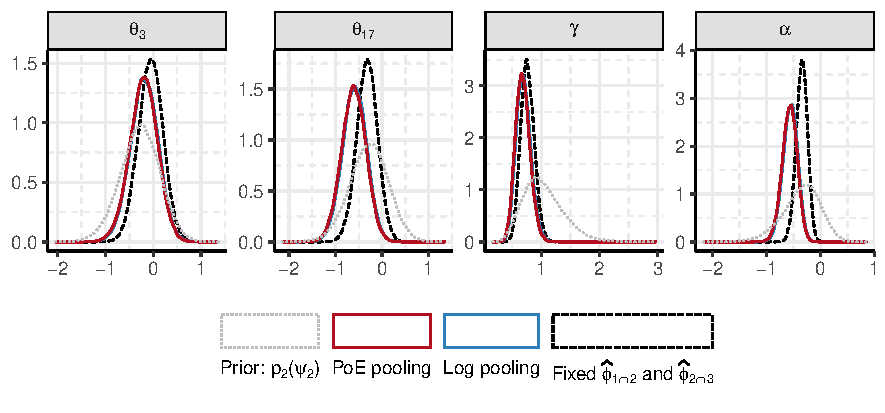
\includegraphics{../plots/mimic-example/psi-2-method-comparison-small} \end{center}

\hypertarget{pooling-the-priors}{%
\section{Pooling the priors}\label{pooling-the-priors}}

Once we have expressions or estimates of the prior marginal
distributions, we need to:

\begin{itemize}
\tightlist
\item
  Decide what type of pooling to use (probably all of them and compare)
\item
  Choose pooling weights, and run some kind of prior predictive check?
\item
  Apportion the pooled prior over the stages of the multi-stage sampler,
  and which stage to divide by the marginals.
\end{itemize}

\hypertarget{cohort-selection-criteria}{%
\section{Cohort selection criteria}\label{cohort-selection-criteria}}

The individuals in our data are included based

\hypertarget{bibliography}{%
\section{Bibliography}\label{bibliography}}

\hypertarget{refs}{}
\begin{CSLReferences}{1}{0}
\leavevmode\hypertarget{ref-belgorodski_rriskdistributions_2017}{}%
Belgorodski, N., Greiner, M., Tolksdorf, K., et al. (2017)
{rriskDistributions}: {Fitting} distributions to given data or known
quantiles.

\leavevmode\hypertarget{ref-beyersmann_simulating_2009}{}%
Beyersmann, J., Latouche, A., Buchholz, A., et al. (2009) Simulating
competing risks data in survival analysis. \emph{Statistics in
Medicine}, \textbf{28}, 956--971. DOI:
\href{https://doi.org/10.1002/sim.3516}{10.1002/sim.3516}.

\leavevmode\hypertarget{ref-brilleman_bayesian_2020}{}%
Brilleman, S. L., Elci, E. M., Novik, J. B., et al. (2020) Bayesian
survival analysis using the rstanarm {R} package. \emph{arXiv:2002.09633
{[}stat{]}}. Available at: \url{http://arxiv.org/abs/2002.09633}.

\leavevmode\hypertarget{ref-kalbfleisch_statistical_2002}{}%
Kalbfleisch, J. D. and Prentice, R. L. (2002) \emph{The Statistical
Analysis of Failure Time Data}. 2nd ed. Wiley series in probability and
statistics. {Hoboken, N.J}: {J. Wiley}.

\leavevmode\hypertarget{ref-soetaert_rootsolve_2020}{}%
Soetaert, K., lsodes.f, A. C. H. (files., sparse.f), et al. (2020)
{rootSolve}: {Nonlinear Root Finding}, {Equilibrium} and {Steady}-{State
Analysis} of {Ordinary Differential Equations}.

\end{CSLReferences}

\renewcommand{\thesection}{\Alph{section}}
\setcounter{section}{0}

\hypertarget{appendix}{%
\section{Appendix}\label{appendix}}

\hypertarget{why-the-censoring-competing-risk-approaches-are-not-the-same}{%
\subsection{Why the censoring / competing risk approaches are not the
same}\label{why-the-censoring-competing-risk-approaches-are-not-the-same}}

Patients who expire or are discharged are not actually censored.
Instead, they experience the competing, non-independent event of
death/discharge.

Suppose that each individual \(i\) experiences one of \(d_{i} = 1, 2\)
competing risks. We observe \(\{T_{i}, d_{i}\}\), where \(d_{i} = 1\)
indicates that individual \(i\) experienced respiratory failure at time
\(T_{i}\). If \(d_{i} = 2\) then individual \(i\) expired or was
discharged at time \(T_{i}\), noting that this event must occur at time
\(C_{i}\). Each cause-specific hazard has parameters \(\theta_{d_{i}}\)
and we denote the hazard
\(h_{i, d_{i}}(t \mid \theta_{d_{i}}, \boldsymbol{w}_{i})\). Denote
\(\boldsymbol{\theta} = (\theta_{1}, \theta_{2})\) and assume only one
such event can occur at a time so that \begin{gather}
  h_{i}(T_{i} \mid \boldsymbol{\theta}, \boldsymbol{w}_{i}) = \sum_{d_{i} \in \{1, 2\}} h_{i, d_{i}}(T_{i} \mid \theta_{d_{i}}, \boldsymbol{w}_{i}), \\
  \begin{aligned}
  H_{i}(T_{i} \mid \boldsymbol{\theta}, \boldsymbol{w}_{i})
    &= \int_{0}^{T_{i}} \sum_{d_{i} \in \{1, 2\}} h_{i, d_{i}}(u \mid \theta_{d_{i}}, \boldsymbol{w}_{i}) \text{d}u \\
    &= \sum_{d_{i} \in \{1, 2\}} \int_{0}^{T_{i}} h_{i, d_{i}}(u \mid \theta_{d_{i}}, \boldsymbol{w}_{i}) \text{d}u \\
    &= \sum_{d_{i} \in \{1, 2\}} H_{i, d_{i}}(T_{i} \mid \theta_{d_{i}}, \boldsymbol{w}_{i}),
  \end{aligned} \\
  S_{i}(T_{i} \mid \boldsymbol{\theta}, \boldsymbol{w}_{i})
    = \exp\left\{-H_{i}(T_{i} \mid \boldsymbol{\theta}, \boldsymbol{w}_{i})\right\}
    = \exp\left\{-\sum_{d_{i} \in \{1, 2\}} H_{i, d_{i}}(T_{i} \mid \theta_{d_{i}}, \boldsymbol{w}_{i})\right\}.
\end{gather} As per Equation (8.8) in
\protect\hyperlink{ref-kalbfleisch_statistical_2002}{Kalbfleisch and
Prentice} (\protect\hyperlink{ref-kalbfleisch_statistical_2002}{2002})
the likelihood function for a specific individual is \begin{align*}
  \pd(T_{i}, d_{i} \mid \boldsymbol{\theta}, \boldsymbol{w}_{i})
    &= h_{i, d_{i}}(T_{i} \mid \theta_{d_{i}}, \boldsymbol{w}_{i}) S_{i}(T_{i} \mid \boldsymbol{\theta}, \boldsymbol{w}_{i}) \\
    &= h_{i, d_{i}}(T_{i} \mid \theta_{d_{i}}, \boldsymbol{w}_{i}) \exp\left\{-\sum_{d_{i} \in \{1, 2\}} H_{i, d_{i}}(T_{i} \mid \theta_{d_{i}}, \boldsymbol{w}_{i})\right\}.
\end{align*}

It is now necessary to assume

\begin{itemize}
\tightlist
\item
  that there are no shared elements in \(\theta_{1}\) and \(\theta_{2}\)
  and they are a priori independent,
\item
  that \(\theta_{2}\) is not of interest, i.e.~we wish to
  integrate/marginalise \(\theta_{2}\) out of the likelihood.
\end{itemize}

The model (given covariates \(\boldsymbol{w}_{i}\)) is

\begin{equation}
  \pd(T_{i}, d_{i}, \boldsymbol{\theta} \mid \boldsymbol{w}_{i}) =
    \pd(T_{i}, d_{i} \mid \boldsymbol{\theta}, \boldsymbol{w}_{i})\pd(\boldsymbol{\theta}).
\end{equation}

We are interested in the following marginal

\begin{equation}
  \pd(T_{i}, d_{i}, \theta_{1} \mid \boldsymbol{w}_{i})
  = \int \pd(T_{i}, d_{i}, \boldsymbol{\theta} \mid \boldsymbol{w}_{i}) \text{d}\theta_{2}
  = \int h_{i, d_{i}}(T_{i} \mid \theta_{d_{i}}, \boldsymbol{w}_{i}) S_{i}(T_{i} \mid \boldsymbol{\theta}, \boldsymbol{w}_{i}) \pd(\theta_{1}) \pd(\theta_{2}) \text{d}\theta_{2}.
\end{equation} If \(d_{i} = 1\) \begin{equation}
  \pd(T_{i}, d_{i}, \theta_{1} \mid \boldsymbol{w}_{i})
  = h_{i, 1}(T_{i} \mid \theta_{1}, \boldsymbol{w}_{i}) S_{i, 1}(T_{i} \mid \theta_{1}, \boldsymbol{w}_{i}) \pd(\theta_{1}) \int S_{i, 2}(T_{i} \mid \theta_{2}, \boldsymbol{w}_{i}) \pd(\theta_{2}) \text{d} \theta_{2},
  \label{eqn:competing-risks-deriv-one}
\end{equation} and if \(d_{i} = 2\) \begin{equation}
  \pd(T_{i}, d_{i}, \theta_{1} \mid \boldsymbol{w}_{i})
  = S_{i, 1}(T_{i} \mid \theta_{1}, \boldsymbol{w}_{i}) \pd(\theta_{1}) \int h_{i, 2}(T_{i} \mid \theta_{2}, \boldsymbol{w}_{i}) S_{i, 2}(T_{i} \mid \theta_{2}, \boldsymbol{w}_{i}) \pd(\theta_{2}) \text{d} \theta_{2}.
  \label{eqn:competing-risks-deriv-two}
\end{equation} Standard survival analyses consider \(T_{i}\) as data.
Under this assumption the integrals in
\eqref{eqn:competing-risks-deriv-one} and
\eqref{eqn:competing-risks-deriv-two} are constants that do not depend
on the parameters of interest, and can be ignored in the
partial-likelihood. The remaining components of
\eqref{eqn:competing-risks-deriv-one} and
\eqref{eqn:competing-risks-deriv-two} comprise the likelihood that would
be obtained by considering all non \(d_{i} = 1\) events as censored.
However, in our case \(T_{i}\) is a parameter, and hence the integrals
are non-ignorable functions of \(T_{i}\).

\begin{itemize}
\tightlist
\item
  If \(d_{i} = 2\), then \(T_{i}\) is `fixed' at \(C_{i}\).
\item
  The type-indicator \(d_{i}\) is now a parameter, where as the
  censoring indicator before was a function of the known length-of-stay
  and the observed event time.
\item
  It's probably easiest to explicitly model the death/discharge event
  and opt for a piecewise constant hazard.

  \begin{itemize}
  \tightlist
  \item
    In this case, the likelihood is really just a mixture of an
    exponential distribution and a Weibull distribution, where the
    covariates only affect the scale parameter of the Weibull
    distribution.
  \end{itemize}
\end{itemize}

\end{document}
